\documentclass[]{interact}
\usepackage{epstopdf}% To incorporate .eps illustrations using PDFLaTeX, etc.
\usepackage[caption=false]{subfig}% Support for small, `sub' figures and tables
%\usepackage[nolists,tablesfirst]{endfloat}% To `separate' figures and tables from text if required
%\usepackage[doublespacing]{setspace}% To produce a `double spaced' document if required
%\setlength\parindent{24pt}% To increase paragraph indentation when line spacing is doubled

\usepackage[numbers,sort&compress]{natbib}% Citation support using natbib.sty
\bibpunct[, ]{[}{]}{,}{n}{,}{,}% Citation support using natbib.sty
\renewcommand\bibfont{\fontsize{10}{12}\selectfont}% Bibliography support using natbib.sty
\makeatletter% @ becomes a letter
\def\NAT@def@citea{\def\@citea{\NAT@separator}}% Suppress spaces between citations using natbib.sty
\makeatother% @ becomes a symbol again

\theoremstyle{plain}% Theorem-like structures provided by amsthm.sty
\newtheorem{theorem}{Theorem}[section]
\newtheorem{lemma}[theorem]{Lemma}
\newtheorem{corollary}[theorem]{Corollary}
\newtheorem{proposition}[theorem]{Proposition}

\theoremstyle{definition}
\newtheorem{definition}[theorem]{Definition}
\newtheorem{example}[theorem]{Example}

\theoremstyle{remark}
\newtheorem{remark}{Remark}
\newtheorem{notation}{Notation}

\usepackage[utf8]{inputenc}
\usepackage{amsmath}
\usepackage{amssymb}
\usepackage[ruled,vlined, linesnumbered]{algorithm2e}
\usepackage[english]{babel}
\usepackage[nottoc]{tocbibind}
\usepackage{xcolor}
\usepackage{graphicx}
\usepackage{float}
\usepackage{hyperref}
\hypersetup{colorlinks=true, citecolor=black, linkcolor=., urlcolor=cyan}
\graphicspath{{../plots/}}

% Custom commands / shortcuts
\providecommand{\sign}{\textrm{sign}}
\providecommand{\pb}[1]{\textcolor{red}{#1}}
\providecommand{\lam}{\lambda}
\newcommand{\quotes}[1]{`#1'}


\title{Adaptive Hybrid Screening for Efficient Lasso Optimization}

\author{Word count: 8899.}

  

\date{}

\begin{document}

\maketitle


\begin{abstract}
Lasso type models are popular in statistics, especially for high-dimensional data. Typical practice is to tune the size of lasso penalty along a path of values. Due to modern data collection techniques, researchers need to analyze data with millions of features, which brings a great need for an efficient lasso optimization algorithm. Feature screening techniques have proven to be powerful for this need, because they can discard features and lead to a model with much less features. In this paper, we develop an adaptive hybrid screening framework where screening is carried out adpatively along the path of tuning parameter values. It reuses previous solutions in the path and reduces unhelpful heavy computations. It is a flexible framework that can be easily extended to different types of lasso models. Two applications for the standard lasso model and the sparse logistic model are shown as examples. We perform simulation study and real data study in a wide range of scenarios and the adaptive hybrid methods outperform other state-of-the-art method significantly and uniformly, with the greatest speedup in the most challenging scenarios.
\end{abstract}

\begin{keywords}
Lasso; feature Screening; safe screening; solution path; large-scale sparse learning
\end{keywords}

\section{Introduction}

The least absolute shrinkage and selection operator, or lasso \citep{tibshirani1996regression}, is a popular model in statistics and machine learning, especially in high-dimensional problems. The model can be defined as the following modification of the least squares optimization problem:
\begin{equation}
  \label{eq:lasso}
  \hat{\beta}(\lambda)=\underset{\beta\in \mathbb{R}^p}{\mathrm{argmin}}\frac{1}{2n}||y-X\beta||_2^2+\lambda||\beta||_1,
\end{equation}
where $y$ is an $n\times 1$ vector of responses, $X=(x_1,x_2,...,x_p)$ is an $n\times p$ matrix of features, $\beta\in \mathbb{R}^p$ is the $p\times 1$ coefficient vector and $\lambda$ is the regularization tuning parameter. Throughout, we use $||\cdot||_2$ denotes the $l_2$ (Euclidean) norm and $||\cdot||_1$ denotes the $l_1$ norm. 

The lasso model has several attractive properties compared to least squares regression, including increased stability of estimation, increased prediction accuracy, and automatic variable selection arising from the fact that it yields sparse estimates of $\beta$.  As a result, it is widely applied in different fields, such as gene expression data analysis, image recognition and text mining, and has been extended in several ways, such as group lasso \citep{yuan2006model}, elastic net \citep{zou2005regularization} and sparse generalized linear models. Because of its wide popularity, solving the lasso efficiently is an important topic in statistics and machine learning.

Because the optimal value of $\lambda$ is not known in advance, typical practice is to solve for $\beta$ along a sequence of values of the tuning parameter $\lambda$, known as the solution path. While efficiently algorithms have been developed \citep{friedman2007pathwise} for the solution path, modern data collection and storage techniques allow researchers to measure an increasingly large number of features, which introduce additional computational challenges. In particular, it may not be possible to store the feature matrix, which can require many GBs of memory to store, in memory. One can resolve this problem by using a memory mapping package such as \textbf{bigmemory}, which allows us to store the feature matrix on disk and read it portions of it as needed; however, this results in frequent reading from disk, which is extremely slow compared to other parts of the algorithm and becomes a bottleneck with respect to the computational burden of fitting lasso models on very large data sets.

One promising technique to address this challenge is feature screening. The lasso model solution is sparse in the sense that most coefficients will be exactly zero; for these \quotes{inactive} coefficients we do not need their associated features.  In theory, if we knew which coefficients were nonzero at each value of $\lambda$, we could read into memory only those features and leave the remaining features on disk. In reality, we cannot know this prior to fitting the model -- however, through the clever use of feature screening rules, we can greatly reduce the number of times inactive features are read into memory, thereby minimizing the computational burden. There are many screening techniques where the solution obtained after screening is guaranteed to be the global optimum if one exists, and in this paper we focus only on this type of screening. In what follows, we refer to features left on disk as \quotes{discarded} features, although it is worth clarifying that this is not a permanent decision.  In particular, a feature can be discarded at one value of $\lambda$ but included in the list of potentially active features at other values of $\lambda$.

There are two important categories of feature screening rules: \quotes{strong} rules \citep{Tibshirani2012, qian2019fast}, which occasionally incorrectly discard some active features, and \quotes{safe} rules \citep{ghaoui2010safe,wang2013lasso,xiang2012fast, xiang2011learning}, which are guaranteed never to do so.  As one might expect, strong rules tend to be easier to calculate; however, because mistakes are possible, one must add a post-convergence check to ensure that no features were incorrectly discarded. This check is not necessary with safe rules. However, safe rules are considerably less powerful at discarding features than strong rules. More recently, hybrid approaches \citep{Zeng2021} combining the two types of rules have been shown to be more efficient than either type of rule alone.

Safe screening rules can be implemented in one of two ways. Sequential rules do screening at each $\lambda$ value along the path using the previous solution as the reference, so they require heavy computation but are relatively powerful. One-step only use the solution at the beginning of the path as the reference. As a result, they require far less computational burden but they lose efficacy as the thus are faster but they cannot remain powerful along the path for long because they don't utilize previous solution.

In this paper, we propose an adaptive safe screening scheme. We begin choosing a solution as the reference for the safe rule and applying it to multiple solution steps along the path. However, unlike the one-step implementation, we monitor the power of the rule with this reference and once it is no longer effective, update the reference of the safe rule to the latest solution.  This process is repeated along the path, waiting until it is beneficial before investing in a new safe rule reference. This scheme avoids disadvantages of both sequential rules and one-step rules. Reusing the same solution as reference when the safe rule is still effective avoids unnecessary computations, while periodically updating the reference ensures that they maintain power across the entire path. We show that this adaptive approach can greatly reduce the computation time and outperforms other methods in all scenarios. Following the hybrid approaches, we also combined our approach with strong rules to form adaptive hybrid rules. Our method is general, and capable of utilizing any sequential safe rule, and thus readily extended to other lasso type models for which safe rules exist. Here, we illustrate its extensions to the logistic regression loss function and to the group lasso penalty.

This manuscript provides a brief review of existing feature screening rules in Section\ref{sec:existing} as well as the following novel contributions:

\begin{itemize}
    \item A new feature screening framework (Section 3.1,3.2), which updates the reference for screening along the grid of $\lambda$ values on any combination of strong screening rules and safe screening rules, which can generate a family of more efficient and scalable screening rules, compared to previous screening rules that are either sequential or one-step.
    \item Three specific applications of this framework, for fitting lasso-penalized linear regression, lasso-penalized logistic regression and group lasso models, respectively (Section~\ref{sec:method},~\ref{sec:logis},~\ref{sec:group}).
    \item An algorithm to determine when to update to a new reference $\lambda$ value for best efficiency (Section \ref{sec:adaptive}).
    \item Simulation studies (Section~\ref{sec:sim}) and real data analysis (Section~\ref{sec:real-data}) under a variety of scenarios, including testing data sets larger than memory, which showed that the proposed algorithms outperform other approaches in all cases, with substantial speed up.
    \item The new feature screening methods for lasso-penalized linear regression and logistic regression were implemented and added as new options to the publicly accessible \textbf{R} package \textbf{biglasso} \citep{zeng2017biglasso}, which was used to carry out the analyses in this manuscript.
\end{itemize}

\section{Existing Feature Screening Rules}
\label{sec:existing}

Throughout this paper, it will be assumed that $y$ is centered and $\{x_j\}_{j=1}^p$ are centered and standardized:
\begin{equation}
  \label{eq:std}
  \sum_{i=1}^ny_i=0, \qquad \sum_{i=1}^n x_{ij}=0, \qquad \sum_{i=1}^n x_{ij}^2=n,\qquad j=1,2,...,p.
\end{equation}
Standardization ensures that the penalty is applied equally to all features, even if originally measured in different units. It also improves the efficiency and stability of the optimization, and helps to simplify optimization.  For example, under this standardization, the intercept is exactly 0 and thus may be ignored.  Standardization also simplifies the formulas for screening rules and thus allows for more efficient implementation.  Furthermore, this can be done without loss of generality as one can always obtain the solution on the original scale through a simple linear transformation of the standardized solution.

Typical practice when fitting lasso models is to solve for $\hat{\beta}(\lambda)$ along a decreasing sequence of $L+1$ values of $\lambda$: $\lambda_0 > \lambda_1 > \cdots > \lambda_L$.  As we discuss shortly, we set $\lambda_0=\max_j|x_j^Ty/n|$ throughout; this ensures that $\hat{\beta}(\lambda_0)=0$, making it a natural point from which to start.

The goal of pathwise algorithms is to solve for this entire solution path.  This can be done efficiently by using \quotes{warm starts}: using previous points on the path as initial values, as these are likely to be relatively close to the solution.  For the model at any $\lambda$-value $\lambda_{l+1}$, letting $r(\lambda_{l+1}) \equiv y-X\hat{\beta}(\lambda_{l+1})$ denote the vector of residuals, the solution $\hat{\beta}(\lambda_{l+1})$ can be computed using the previous solution $\hat{\beta}(\lambda_l)$ as the initial value in the algorithm. Pathwise coordinate descent is a algorithm that takes advantage of this idea and will be used as the lasso algorithm for the rest of the paper.

In convex optimization, the Karush-Kuhn-Tucker (KKT) conditions are both necessary and sufficient for any optimal solution.  Screening rules take advantage of these KKT conditions in order to discard inactive coefficients.  For the lasso, the KKT conditions governing the optimal solution $\hat{\beta}(\lambda)$ are given by
\begin{equation}
  \label{eq:kkt}
  \begin{aligned}
    x_j^Tr(\lambda)/n &= \lambda \, \sign \, \hat{\beta}_j(\lambda) & & \textrm{if } \hat{\beta}_j(\lambda)\neq 0,\\
    |x_j^Tr(\lambda)/n| &\leq \lambda & & \textrm{if } \hat{\beta}_j(\lambda)= 0.
  \end{aligned}
\end{equation}
If the residuals were known, we could safely conclude that $\hat{\beta}_j(\lambda)=0$ by verifying that the second condition holds as a strict inequality.  The complication, of course, is that the residuals are not known until after we have solved for all the coefficients.  However, when fitting a solution path, residuals at previous $\lambda$ values provide information about residuals at the next $\lambda$ value and thus may be used for screening. Note that if we have $\lambda_0=\max_j|x_j^Ty/n|$ and $\hat{\beta}(\lambda_0)=0$, then $r(\lambda_0)=y$ satisfies the KKT conditions and thus $\hat{\beta}(\lambda_0)=0$ is the optimal solution.

\subsection{Active-set Cycling}
\label{sec:active}

The simplest of all screening rules is to simply assume that features currently in the model will stay in the model and features currently excluded will remain excluded.  This is known as active-set cycling (AC) \citep{lee2007efficient}. It can be implemented on top of any lasso algorithm with no additional cost. When solving the coefficients for at $\lambda_{l+1}$, AC considers only features whose coefficients were non-zero at $\lambda_l$ and discards the other features. The lasso problem is then solved over this reduced number of coefficients.

After computing the solution, a post-convergence KKT conditions check is performed. Because the KKT conditions are sufficient for the solution to be optimal, if there is no violation, the solution to the smaller model will be exactly the same as if we solve the model with all features. If there are violations, corresponding features will be added to the model and this procedure is repeated. There are a finite number of features that can be added, so the procedure will end after finite repetitions. Because features enter the model relatively infrequently, typically only a small number of repetitions are needed, thereby providing a substantial speed up compared to solving the full lasso problem every time.

\subsection{Strong Rules}

Each post-convergence check requires $O(np)$ operations and is therefore costly to repeat when violations occur.  These violations are inevitable in active-set cycling, as they occur every time a feature is added to the model.  Sequential strong rules (SSR) \citep{Tibshirani2012} have the basic idea of active-set cycling, but reduce violations by retaining features that are \quotes{close} to entering the model.

Given the solution $\hat{\beta}(\lambda_l)$ and residual vector $r(\lambda_l)=y-X\hat{\beta}(\lambda_l)$ at $\lambda_l$, the SSR discards the $j$-th feature at $\lambda_{l+1}$ if:
\begin{equation}
  \label{eq:ssr}
  |x_j^Tr(\lambda_l)/n|<2\lambda_{l+1}-\lambda_l.
\end{equation}
The SSR is derived from the KKT condition and the \quotes{unit-slope} assumption that the size of the slope of $x_j^Tr(\lambda)/n$ over $\lambda$ is bounded by 1. 

The biggest problem of SSR is that the \quotes{unit-slope} assumption may not hold and thus discarded features are not guaranteed to have zero coefficients. As with AC, a post-convergence KKT check is therefore needed for the discarded features to make sure their coefficients are truly zero. If violations occur, we again need to refit the model, adding the violating features and repeating the post-convergence check. Similar to the procedure in AC, there are a finite number of features that can be added, so the procedure will end after finite repetitions. Moreover, previous studies have shown that violations are rare, so the additional $O(np)$ cost for repeating a KKT check hardly ever arises.

SSR possesses the nice property that the quantity $x_j^Tr(\lambda_l)/n$ needed for SSR screening \eqref{eq:ssr} at $\lambda_{l+1}$ has already been calculated during post-convergence checking at $\lambda_l$ in \eqref{eq:kkt}. As this is the only computationally intensive aspect of SSR screening, and SSR violations are rare, its computational cost is roughly $O(npL)$.

\subsection{Safe Rules}
\label{sec:safe}

Compared to strong rules, safe rules are never violated. Features can be discarded safely, with no need for post-covergence checking, as the coefficients are guaranteed to be zero by the rule. We mainly focus on enhanced dual polytope projections (EDPP) rules\citep{wang2013lasso} because they outperform other known safe rules and are easy to incorporate into our method.

The EDPP rules are derived from the dual formulation of the lasso problem and provide a bound for the residual vector $r(\lambda)$. Then using the KKT conditions, some features can be guaranteed to have zero coefficients and be discarded safely. Two forms of the EDPP rule, basic EDPP (BEDPP) and sequential EDPP (SEDPP)\citep{wang2013lasso}, were proposed and under the standardization \eqref{eq:std} can be simplified in the following theorems \citep{Zeng2021}:

\begin{theorem}[BEDPP]
    For the lasso problem \eqref{eq:lasso}, let $\lambda_0:=\max_j|x_j^Ty/n|$ and $x_*=\arg \max_{x_j}|x_j^Ty/n|$. Under \eqref{eq:std} and for any $\lambda\in(0,\lambda_0]$, we have $\hat{\beta}_j(\lambda)=0$ if
    \begin{equation}
        \label{eq:bedpp}
        |(\lambda_0+\lambda)x_j^Ty-(\lambda_0-\lambda)sign(x_*^Ty)\lambda_0x_j^Tx_*|<2n\lambda_0\lambda-(\lambda_0-\lambda)\sqrt{n||y||_2^2-n^2\lambda_0^2}.
    \end{equation}
\end{theorem}

\begin{theorem}[SEDPP]
    For the lasso problem \eqref{eq:lasso}, let $\lambda_0:=\max_j|x_j^Ty/n|$. Suppose we have a sequence of $\lambda$ values $\lambda_0>\lambda_1>...>\lambda_L$. Under condition \eqref{eq:std}
    \begin{enumerate}
        \item For any $l=1,2,...,L-1$, given $\hat{\beta}(\lambda_l)$, $r(\lambda_l)$ and $\hat{y}(\lambda_l):=X\hat{\beta}(\lambda_l)$, then $\hat{\beta}_j(\lambda_{l+1})=0$ if
        \begin{equation}
            \label{eq:sedpp}
            \begin{split}
                &\left|2\lambda_{l+1}x_j^Tr(\lambda_l)+(\lambda_l-\lambda_{l+1})\left( x_j^Ty-\frac{y^T\hat{y}(\lambda_l)x_j^T\hat{y}(\lambda_l)}{||\hat{y}(\lambda_l)||_2^2}\right)\right|\\&<2n\lambda_l\lambda_{l+1}-(\lambda_l-\lambda_{l+1})\sqrt{n||y||_2^2-\frac{n(y^T\hat{y}(\lambda_l))^2}{||\hat{y}(\lambda_l)||_2^2}}
            \end{split}
        \end{equation}
        \item For l=0, i.e., $\lambda_l=\lambda_0$, SEDPP rule reduces to BEDPP rule. $\hat{\beta}_j(\lambda_1)=0$ if \eqref{eq:bedpp} holds with $\lambda=\lambda_1$.
    \end{enumerate}
\end{theorem}

In BEDPP rule \eqref{eq:bedpp}, the most costly parts of computation that take $O(np)$ time are the computation of $\{x_j^Ty\}_{j=1}^p$ and $\{x_j^Tx_*\}_{j=1}^p$ ($x_*^Ty$ is an element of $\{x_j^Ty\}_{j=1}^p$). These quantities do not depend on $\lambda_l$ and thus only need to be computed once at the beginning and stored. After this step, other computation of the rule takes almost zero time, so BEDPP rule can be viewed as an one-step rule with $O(np)$ cost.

In contrast, the SEDPP rule \eqref{eq:sedpp} requires $\{x_j^Tr(\lambda_l)\}_{j=1}^p$, which must be recomputed at every $\lam$.  This is the primary source of computational burden, as the other terms in the rule are $\{x_j^Ty\}_{j=1}^p$, which only needs to be calculated once, and $x_j^T\hat{y}(\lambda_l)$, which can be computed as $x_j^Ty-x_j^Tr(\lambda_l)$. Thus, the sequential safe rule SEDPP requires $O(npL)$ operations.

Comparing the two, BEDPP is much faster, but at each $\lambda_l$, it is bounding $r(\lambda_l)$ using $r(\lambda_0)=y$ as a reference. As $\lambda_l$ gets further away from $\lambda_0$, this bound becomes less precise and the screening rule becomes less powerful. SEDPP is slower, but at each $\lambda_{l+1}$, it uses $r(\lambda_{l})$ as the reference. Because $\lambda_{l+1}$ and $\lambda_l$ are close, the bound remains tight and screening continues to be powerful over the entire path.

\subsection{Other Approaches to Screening}

Hybrid safe-strong rules (HSSR) \citep{Zeng2021} were proposed to combine SSR with any safe rule, thereby taking advantage of both. Specifically, they recommended combining SSR with BEDPP rule, which showed the greatest efficiency in experiments. This algorithm discards features that are discarded by either SSR or BEDPP rule. Then, during the post-convergence check, it checks only those features discarded by SSR but not by BEDPP, as the latter can be safely discarded and do not need post-convergence checking. By doing so, the hybrid approach greatly reduces the computational burden of post-convergence KKT checking.  As shown in that paper, hybrid rules combine the advantages of each type of rule, and result in an algorithm that is faster than either strong or safe rules alone.

Batch screening iterative lasso (BASIL) \citep{qian2019fast} was proposed to carry out SSR screening and post-convergence checking in batches. Suppose we have a previous solution $\hat{\beta}(\lambda_l)$ and $r(\lambda_l)$ and the batch of $\{\lambda_{l+1},\lambda_{l+2},...,\lambda_{l+B}\}$ values we are going to solve at. First, screening is carried out for each $\lambda_{l+b}$ in the batch based $r(\lambda_l$ by discarding the $j$th feature if $|x_j^Tr(\lambda_l)/n|<2\lambda_{l+b}-\lambda_l$. The lasso problem is then solved for $\lam$ values in the batch using only features that are not discarded. Finally, during post-convergence checking, we search for last $l+b$ in the batch $\{l+1,l+2,...,l+B\}$ such that the KKT conditions hold at $\lambda_{l+b}$ and accept only the solutions from $\lambda_{l+1}$ to $\lambda_{l+b}$. Next, we move to a new batch by replacing the batch head $l$ with $l+b$ and repeat the same procedure again.

BASIL is most beneficial when $X$ is to large to be fit into the RAM, as it minimizes the amount of time spent reading from disk. During post-convergence checking, each $x_j$ only needs to be read in once for the entire batch and can be used multiple times for $\{\lambda_{l+1},\lambda_{l+2},...,\lambda_{l+B}\}$. Moreover, similar to SSR, the $x_j^Tr(\lambda_{l+b})$ values computed at BASIL's post-convergence check can be reused for screening at next batch.

In addition to the deterministic screening methods we have described, there are also probabilistic screening rules such as Sure Independence Screening \citep{Fan2008}. In this paper, we consider only screening methods that never falsely discard an active feature and that are thus guaranteed to converge to the global solution. This is not the case for probabilistic screening approaches, which construct screening rules such that the probability of incorrectly discarding active features tends to 0 asymptotically under certain conditions, but for any finite sample size, have a positive probability of converging to an inferior solution.

\section{Adaptive Screening}
\label{sec:method}

% In this section, we will introduce the framework of adaptive hybrid rules, implement them with EDPP as the safe rule to form Ada-SSR-EDPP and propose a strategy to adaptively updating the reference.

\subsection{Adaptive Safe Rules}

The SEDPP rule \eqref{eq:sedpp} from Theorem 2.2 allows us to screen features at $\lambda_{l+1}$ using the solution at $\lambda_l$ as a reference. However, since the grid of $\lam$ values is arbitrary, the rule with the same reference can be just as easily applied to screen solutions at $\lam_{l+2}, \lam_{l+3}, \ldots$, until some $\lam_{l+B}$, where we update the reference to the current solution at $\lam_{l+B}$ and screen the following $\lam$ values.  The difference is that in typical SEDPP usage, we would update the reference solution at every step of path; here, we are proposing to re-use solutions for several values of $\lam$, only updating the reference when it is computationally beneficial to do so.  We refer to this modification as \emph{adaptive EDPP}.  Adaptive EDPP is still a safe rule, but it is neither sequential nor one-step.   A similar idea would be to use the reference solution in batches, each one being used for a fixed number of $\lam$ steps.  However, since an appropriate batch size is difficult to determine ahead of time, and also because the ideal size changes along the path, we find that an adaptive approach is better (see Section~\ref{sec:adaptive}).

The Adaptive EDPP rule can be stated in the following theorem, which simply restates the theorems from Section~\ref{sec:safe} in terms of this new paradigm in which a single reference solution at $\lam_l$ is used to calculate screening rules at $\lam_{l+1}, \ldots, \lam_{l+B}$.

\begin{theorem}[Adaptive EDPP]
    For the lasso problem \eqref{eq:lasso}, let $\lambda_0:=\max_j|x_j^Ty/n|$. Suppose we have a sequence of $\lambda$ values $\lambda_0>\lambda_1>...>\lambda_L$ and the last updated reference point is $\lambda_l$. Under condition \eqref{eq:std}
    \begin{enumerate}
        \item For any $l=1,2,...,L-1$, given $\hat{\beta}(\lambda_l)$, $r(\lambda_l)$ and $\hat{y}(\lambda_l):=X\hat{\beta}(\lambda_l)$, then for some next update point $l+B$ and any $b$ s.t. $l<l+b\leq l+B\leq L$, $\hat{\beta}_j(\lambda_{l+b})=0$ if
        \begin{equation}
            \label{eq:aedpp1}
            \begin{split}
                &\left|2\lambda_{l+b}x_j^Tr(\lambda_l)+(\lambda_l-\lambda_{l+b})\left( x_j^Ty-\frac{y^T\hat{y}(\lambda_l)x_j^T\hat{y}(\lambda_l)}{||\hat{y}(\lambda_l)||_2^2}\right)\right|\\&<2n\lambda_l\lambda_{l+b}-(\lambda_l-\lambda_{l+b})\sqrt{n||y||_2^2-\frac{n(y^T\hat{y}(\lambda_l))^2}{||\hat{y}(\lambda_l)||_2^2}}
            \end{split}
        \end{equation}
        \item For l=0, i.e., $\lambda_l=\lambda_0$, then for some next update point $B$ and any $b$ s.t. $0<b\leq B\leq L$, $\hat{\beta}_j(\lambda_{b})=0$ if
        \begin{equation}
            \label{eq:aedpp2}
            |(\lambda_0+\lambda_b)x_j^Ty-(\lambda_0-\lambda_b)sign(x_*^Ty)\lambda_0x_j^Tx_*|<2n\lambda_0\lambda_b-(\lambda_0-\lambda_b)\sqrt{n||y||_2^2-n^2\lambda_0^2}.
        \end{equation}
    \end{enumerate}
\end{theorem}

For each $\lambda$ value in $\lambda_{l+1},...,\lambda_{l+B}$, the computation in \eqref{eq:aedpp1} or \eqref{eq:aedpp2} is the same, except for the quantity $\lambda_{l+b}$ ($\lambda_b$ in the case $l=0$). The expensive computations in calculating these rules are $x_j^Tr(\lambda_l)$, $x_j^Tx_*$ and $x_j^Ty$, all of which must be calculated for $j=1,2,...,p$ and thus require $O(np)$ operations; all other computations require at most $O(p)$ operations. However, since $x_j^Ty$ and $x_j^Tx_*$ are the same for all $\lambda$ values and $x_j^Tr(\lambda_l)$ is the same for all $\lambda$ values within the block, once they have been calculated once, they can be stored and reused to avoid additional computation for all remaining steps in the block.  Note that $x_j^T\hat{y}(\lambda_l)=x_j^Ty-x_j^Tr(\lambda_l)$, so this term also can be calculated efficiently.

Compared to one-step methods like BEDPP, the reference solutions are continually updated.  As a result, the reference is always relatively close to the solution, and screening remains powerful over the entire path, unlike one-step methods where screening power drops drastically as $\lambda_l$ gets further away from $\lambda_0$. Compared to sequential methods like SEDPP, the adaptive method only requires $O(np)$ computations per update, while SEDPP requires $O(np)$ computations for each $\lambda$ value. The framework of adaptive safe screening can also be easily applied to other sequential safe rules, to form a family of adaptive safe rules.

\subsection{Adaptive Hybrid Rules}

Since HSSR \citep{Zeng2021} has been shown to provide significant speedup compared to safe rules alone, we also consider incorporating strong rules into adaptive EDPP screening, forming an adaptive hybrid rule combining SSR and adaptive EDPP.

This combination is not trivial. For ordinary SSR, the quantity $x_j^Tr(\lambda_l)$ used in \eqref{eq:ssr} is already computed in the previous post-convergence check in \eqref{eq:kkt}. However, when combined with safe rules, the post-convergence check is not applied to all features. For any feature that was safely discarded at the previous $\lambda$, but not the current $\lambda$, the quantity $x_j^Tr(\lambda_l)$ has not been computed yet and thus cannot be used without additional cost. Similar to the idea of BASIL \citep{qian2019fast}, we can also do the strong rule screening adaptively by using the latest $x_j^Tr(\lambda_l)$ available, which is computed by adaptive EDPP rule at the latest update, to reduce the number of required computations.

We combine adaptive EDPP and SSR to form the adaptive hybrid rule as follows. Let $\lambda_l$ denote the point in the path at which the EDPP reference has been most recently updated, and we want the solution at $\lambda_{l+b}$. First, carry out adaptive EDPP screening. Second, apply adaptive SSR screening to the features that have not been discarded by adaptive EDPP and discard any feature that satisfies $|x_j^Tr(\lambda_l)/n|<2\lambda_{l+b}-\lambda_l$. Third, conduct a post-convergence check on the features that were discarded by adaptive SSR but not discarded by adaptive EDPP. This procedure is then repeated for $\lambda_{l+b+1}$ (unless an EDPP update is applied).

By choosing the same reference for adaptive EDPP rule and adaptive SSR, the quantity $x_j^Tr(\lambda_l)$ only needs to be computed once and can be used by both rules. Also, because the adaptive EDPP rule remains powerful, the set of features that require post-convergence checking remains small.  This is unlike the original hybrid rules using basic EDPP, where the loss of power in EDPP screening for $\lambda \ll \lambda_0$ leads to expensive post-convergence checking.

\subsection{Pathwise Lasso Algorithm with Adaptive Hybrid Rule}

Below, we provide the explicit algorithm used to solve for the lasso solution path using our proposed adaptive hybrid screening rule. For the numeric experiments in Section~\ref{sec:experiments}, this algorithm was implemented using pathwise coordinate descent, but the algorithm can use any algorithm for solving the lasso problem.  Likewise, any adaptive safe rule could be substituted in place of EDPP screening.  Note here the first reference chosen will be $\lambda_0$, where the residuals vector $r(\lambda_0)$ is just the response $y$, because all the $\hat{\beta}(\lambda_0)$ are zero. The quantity $\{x_j^Ty\}_{j=1}^p$ is therefore computed at the beginning and stored for the whole path.

\begin{algorithm}[H]
  \label{alg:path}
    \SetKwInOut{Input}{Input}\SetKwInOut{Output}{Output}\SetKwInOut{Pre}{Pre-compute}\SetKwInOut{Initialize}{Initialize}
    \SetAlgoLined
    \Input{$\{x_j\}_{j=1}^p, \{x_j^Ty\}_{j=1}^p,  \lambda_{0},...,\lambda_{L}$}
    \BlankLine
    \Initialize{reference = $\lambda_0$}
    
    \For{$l\xleftarrow{}$ 1 \KwTo L}{
        Safe Screening: $\mathcal{S}_{l}\xleftarrow{}\{j:x_j$ not discarded by adaptive EDPP rule given the reference$\}$.
        
        Strong Screening: $\mathcal{R}_{l}\xleftarrow{}\{j\in \mathcal{S}_{l}:x_j$ not discarded by adaptive SSR given the reference$\}$.
        
        \Initialize{$\hat{\beta}(\lambda_{l})=\hat{\beta}(\lambda_{l-1}), r(\lambda_{l})=r(\lambda_{l-1})$}
        
        \Repeat{Post-convergence check passes}{
            Solve lasso problem using only features in $\mathcal{R}_{l}$, with warm start $\hat{\beta}(\lambda_{l}), r(\lambda_{l})$. 
            
            Save new $\hat{\beta}(\lambda_{l}), r(\lambda_{l})$.
            
            Post-convergence check for all $j\in \mathcal{S}_{l}\setminus\mathcal{R}_{l}$,
            
            \uIf{Post-convergence check does not pass}{
                Add violating features to $\mathcal{R}_{l}$\;
            }
        }
        \uIf{Update conditions met}{
            Reference = $\lambda_{l}$
            
            Compute and save: $\{x_j^Tr(\lambda_l)\}_{j=1}^p, \{x_j^T\hat{y}(\lambda_l)=x_j^Ty-x_j^Tr(\lambda_l)\}_{j=1}^p, \hat{y}(\lambda_l)=y-r(\lambda_l)$.}
            
    }
    \Output{$\{\hat{\beta}(\lambda_{l})\}_{l=1}^L$}
    \caption{Pathwise lasso algorithm with adaptive hybrid rule screening}
\end{algorithm}

\subsection{Adaptive Update Algorithm}
\label{sec:adaptive}

In this section we will fill in line 11 in Algorithm~\ref{alg:path}. We develop an algorithm to determine when to update the reference for screening. This decision is guided by evaluating screening power at previous $\lambda$ values, and is therefore adaptive, updating the reference more or less frequently as we continue along the solution path. Our goal is to minimize the computation cost, so we will first analyse computation complexity for each part in Algorithm~\ref{alg:path}. Then we will propose an adaptive algorithm that can minimize the entire computation cost.

\subsubsection{Complexity Analysis}
\label{sec:complexity}

This complexity analysis will only consider calculations with $O(np)$ complexity. The remaining calculations, those with $O(p)$ complexity for example, are not only of lower order, but also consume less memory and thus usually do no require out-of-core computing. Calculation of $\{x_j^Ty\}_{j=1}^p$ is needed only once for the whole solution path; we ignore this as well as its computational cost is the same across all approaches. We assume that strong rule screening is always powerful in the sense that its set of non-discarded features, $\mathcal{R}_{l+b}$, satisfies $|\mathcal{R}_{l+b}|=o(p) \approx 0$, but that safe rule screening, with corresponding set $\mathcal{S}_{l+b}$, may not be. We also assume that post-convergence check will usually pass in the first iteration and thus is only needed approximately once per $\lambda$.

Under these assumptions, there are two dominating parts in the algorithm within each update. First, the computation of $\{x_j^Tr(\lambda_l)\}_{j=1}^p$ at the time of updating the reference, which requires $np$ multiplications. Then, for each $\lambda_{l+b}$, the post-convergence check requires approximately $|\mathcal{S}_{l+b} \setminus \mathcal{R}_{l+b}| \approx |\mathcal{S}_{l+b}|$ KKT condition checks, each of which requires $n$ multiplications. These sum to $n\sum_{b=1}^{B}|\mathcal{S}_{l=b}|$ multiplications, where $l+B$ is the start of the next update. Combining these two parts, the average cost per $\lambda$ in the block $\lambda_{l+1},...,\lambda_{l+B}$ is
\begin{equation}
    \label{eq:cost}
    \bar{T}_l(B) \approx n\frac{p}{B}+n\frac{\sum_{b=1}^B|\mathcal{S}_{l+b}|}{B},
\end{equation}
where the first term represents the cost of updating the safe screening rule and the second term the cost of KKT checking. Delaying the next update (increasing $B$) means reusing calculations additional times, thus reducing the cost of safe screening (first term). However, reusing an old reference reduces the power of the safe rule, thereby increasing the cost of KKT checking (second term).

To better illustrate these two effects, we considered a simple updating scheme: update the reference after every batch of $B$ $\lambda$ values. Figure~\ref{fig:batchsizes} illustrates the effect of the batch size $B$ on $|\mathcal{S}_{l+b}|$ in a real data set solved over a path of $L=100$ $\lambda$-values. The vertical axis is the proportion of discarded features, $1-|\mathcal{S}_{l+b}|/p$.

\begin{figure}[ht]
    \centering
    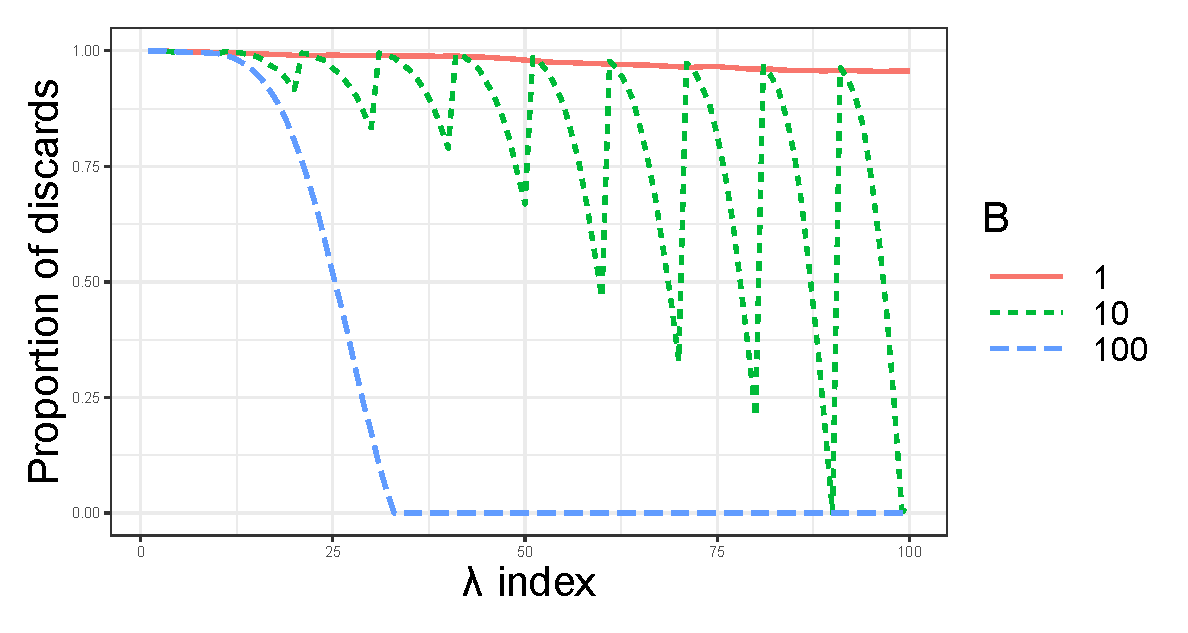
\includegraphics[width=0.6\textwidth]{batchsizes.eps}    \caption{Proportion of features rejected by screening rules vs index of $\lambda$-values for different update delay.}
    \label{fig:batchsizes}
\end{figure}

BEDPP is the special case of adaptive EDPP that never updates ($B=L$). When the reference is not updated, safe rule screening will eventually fail to discard any features and the KKT condition checking cost will increase to its maximum, $np$. SEDPP is the special case that updates at every $\lambda$ value ($B=1$). It remains very powerful along the path, making the KKT condition checking cost small, but safe screening updates themselves are costly and require $np$ operations at every $\lambda$-value. Adaptive EDPP can strike a balance between BEDPP and SEDPP. In this example, simply using a fixed batch size $B=10$ can reduce the safe rule updating cost by 90\% compared to SEDPP and reduce the KKT checking cost by about 80\% compared to BEDPP.

This example also illustrates the appeal of choosing updates in an adaptive manner. For the first 10 $\lambda$ values, the safe rule stays powerful, which means the old reference is still useful. In this portion of the solution path, we want to delay the update in order to reduce the cost of safe screening, with little harm to the cost of KKT condition checking. For the last 20 $\lambda$ values however, the reference quickly becomes useless. In this portion of the solution path, we want to update more frequently in order to reduce the KKT condition checking cost. Moreover, the performance of adaptive EDPP depends on many factors such as the data, the range of $\lambda$-values and spacing between $\lambda$-values. Thus, simply updating the EDPP reference after a fixed batch size will not be as efficient as a method that can adaptively determine whether or not to update.

\subsubsection{Efficient Updating Algorithm}

As explained in the previous section, it is reasonable to assume that the average cost, as a function of the update delay $B$, decreases at first, then reaches an optimal value before it begins increasing again. A reasonable approach to minimizing the average cost, therefore, is to update the reference at the point where reusing it one additional time would increase the average cost. That is, we should update the reference at $\lambda_{l+B}$ if $\bar{T}_l(B+1)>\bar{T}_l(B)$. In practice, we will instead update the reference to $\lambda_{l+B}$ when $\bar{T}_l(B)>\bar{T}_l(B-1)$, because $\bar{T}_l(B+1)$ cannot be calculated without having already carried out screening at $\lambda_{l+B+1}$. The two conditions should be close and thus this substitution should be near optimal. Combined with \eqref{eq:cost}, the latter condition is approximately

\begin{equation}
    \label{eq:crit}
    (B-1)|\mathcal{S}_{l+B}|-\sum_{b=1}^{B-1}|\mathcal{S}_{l+b}|>p.
\end{equation}


This updating condition is a greedy condition that only considers the cost up to the current $\lambda$ value. This is unavoidable in practice, as we cannot know about future $\lambda$ values. The resulting adaptive rule, \eqref{eq:crit}, provides a robust strategy that addresses the three most common scenarios. First, if the screening power stays high, meaning $\mathcal{S}_{l+b}$ is small for all $b$, then the left-hand-side of \eqref{eq:crit} will be small and thus at this point we will not update to further exploit the old reference. Second, if the screening power has been high for a while but dropped suddenly, meaning $\mathcal{S}_{l+B}$ is large but $\mathcal{S}_{l+b}$ are mostly small for $b=1,2,...,B-1$, then the left-hand-side of \eqref{eq:crit} will be large and we will update the useless old reference to a helpful new one. Last, if the screening power drops dramatically immediately after the last update, meaning $\mathcal{S}_{l+b}$ are close to $p$ for $b=2,3,...,B$, then the left-hand-side of \eqref{eq:crit} will be approximately $p-|\mathcal{S}_1|$. This is less than $p$, so we will again not update.  Although the old reference is useless, there is little point in calculating a new reference because if we did, it would quickly become useless as well.

We use this updating condition at line 11 in Algorithm~\ref{alg:path} to form a complete pathwise lasso algorithm with adaptive hybrid screening. 

\section{Extension to other Lasso Type Problems}
\label{sec:extension}

The structure of the adaptive hybrid rule is easily extendable to any lasso problems that have corresponding sequential strong and safe rules. After an adaptive safe rule is built, we can automatically apply the adaptive strong rule and adaptive update algorithm to form a pathwise algorithm with adaptive hybrid screening. Here, we derive extensions to two lasso-type problems and show these extensions improve computation efficiency.

\subsection{Adaptive Safe Rule for Sparse Logistic Regression}
\label{sec:logis}

Consider the sparse logistic regression model where estimates of the coefficient vector $\beta$ and intercept $\beta_0$ are obtained by minimizing
\begin{equation}
    \label{eq:logis}
    %\hat{\beta}(\lambda)=\underset{(\beta,\beta_0)\in \mathbb{R}^p\times\mathbb{R}^1}{\mathrm{argmin}}-
  \frac{1}{n} \sum_{i=1}^n \big\{y_i\log\pi_i(\beta) + (1-y_i)\log(1 -\pi_i(\beta))\big\} + \lambda||\beta||_1,
\end{equation}
where $\pi(\beta)=\{\pi_i(\beta)\}_{i=1}^n=\{p(y_i=1|x_{i1},x_{i2},...,x_{ip})\}_{i=1}^n=\{e^{\eta_i(\beta)}/(1+e^{\eta_i(\beta)})\}_{i=1}^n$ is the predicted value vector and $\eta(\beta)=X\beta+\beta_0\mathbf{1}$ is the linear function. The quantity $X$ is still the $n\times p$ standardized feature matrix but in this model $y\in\{0,1\}^n$ is an unstandardized binary response vector; unlike linear regression, the intercept cannot be eliminated through centering in logistic regression.

Sequential strong rules require only a small change for logistic regression. The residual vector now is $r(\lambda_l)=y-\pi(\hat{\beta}(\lambda_l))$. Then the SSR discards the $j$-th feature at $\lambda_{l+1}$ if \eqref{eq:ssr} holds.

Safe rules require more significant modification, as EDPP no longer applies. In its place, we use Slores \citep[sparse logistic regression screening rule,][]{wang2014safe}. It was proposed as a one-step rule but can be extended to an adaptive rule with minimal changes. 

\begin{theorem}[Adaptive Slores]
For the sparse logistic regression model \eqref{eq:logis}, let $\lambda_0:=\max_j|x_j^Ty/n|$, $\Tilde{y}=2y-1\in\{-1,1\}^n$, and suppose $\lambda_0>\lambda_1>...>\lambda_L$. For all $\theta\in(0,1)^n$, let 

\begin{equation}
    \begin{split}
        g(\theta)&=\frac{1}{n}\sum_{i=1}^n\{\theta_i\log \theta_i+(1-\theta_i)\log(1-\theta_i)\},\\
    \nabla g_i(\theta) &= \frac{1}{n}\log\frac{\theta_i}{1-\theta_i}.
    \end{split}
\end{equation}

Under the conditions on $X$ given in \eqref{eq:std}, for any $l=1,2,...,L-1$, assume $\hat{\beta}(\lambda_l)$, $r(\lambda_l)=y-\pi(\hat{\beta}(\lambda_l))$, $x_*\in\{x_j:\hat{\beta}_j(\lambda_l)\neq0\} $, $\theta(\lambda_l)=\{r_i(\lambda_l)\Tilde{y}_i\}_{i=1}^n$ and $\hat{y}(\lambda_l):=\pi(\hat{\beta}(\lambda_l))$ are known. For some next update point $l+B$ and any $b$ s.t. $l<l+b\leq l+B\leq L$, let
\begin{equation}
  R(\lambda_{l+b}) = \sqrt{\frac{n}{2} \bigg[g\bigg(\frac{\lambda_{l+b}}{\lambda_l}\theta(\lambda_l)\bigg) - g\bigg(\theta(\lambda_l)\bigg) + \bigg(1 - \frac{\lambda_{l+b}}{\lambda_l}\bigg) \bigg(\nabla g\big(\theta(\lambda_l)\big)\bigg)^T\theta(\lambda_l)\bigg]},
\end{equation}
and $d(\lambda_{l+b})=\sqrt{n}(\lambda_l-\lambda_{l+b})/R(\lambda_{l+b})$. For $\xi = -1,1$ and $j=1,2,...,p$,

\begin{enumerate}
    \item If $-\xi \sign(x_*^Ty)x_j^Tx_*\geq nd(\lambda_{l+b})$, then
    
    \begin{equation}
        T_\xi(\lambda_{l+b},x_j;r(\lambda_l))=\sqrt{n}R(\lambda_{l+b})-\xi x_j^Tr(\lambda_l);
    \end{equation}
    
    \item If $-\xi \sign(x_*^Ty)x_j^Tx_*< nd(\lambda_{l+b})$, then
    
    \begin{equation}
        T_\xi(\lambda_{l+b},x_j;r(\lambda_l))=R(\lambda_{l+b})\sqrt{n+nu_\xi^2-2\xi u_\xi \sign(x_*^Ty)x_j^Tx_*}-nu_\xi(\lambda_l-\lambda_{l+b})-\xi x_j^Tr(\lambda_l),
    \end{equation}
    where
    \begin{align}
        u_\xi&=\frac{-\xi a_1+\sqrt{\Delta}}{2a_2},\\
        a_0&=(x_j^Tx_*)^2-n^2d^2(\lambda_{l+b}),\nonumber\\
        a_1&=-2n\,\sign(x_*^Ty)x_j^Tx_*\big(1-d^2(\lambda_{l+b})\big),\nonumber\\
        a_2&=n^2\big(1-d^2(\lambda_{l+b})\big),\nonumber\\
        \Delta&=a_1^2-4a_0a_1.\nonumber
    \end{align}
\end{enumerate}

Then $\hat{\beta}_j(\lambda_{l+b})=0$ if
  \begin{equation}
    \max_{\xi=\pm1} T_\xi(\lambda_{l+b},x_j;r(\lambda_l))<n\lambda_{l+b}
  \end{equation}
\end{theorem}

When computing the adaptive Slores, $\{x_j^Ty\}_{j=1}^p$ needs to be computed only once, after which it can be stored and reused for the whole solution path. The quantity $\{x_j^Tx_*\}_{j=1}^p$ can be similarly reused unless $x_*$ changes, which happens if the corresponding regression coefficient drops out of the model; this is relatively rare, but can happen. Other than those two terms, the only term that requires expensive $O(np)$ computations is $\{x_j^Tr(\lambda_l)\}_{j=1}^p$, which needs to be computed only when we update the reference solution. Thus Algorithm~\ref{alg:path} can be applies to the sparse logistic model, with Slores replacing EDPP, to form the adaptive hybrid rule algorithm for sparse logistic regression.

\subsection{Adaptive Safe Rule for Group Lasso}
\label{sec:group}

The group lasso model \citep{yuan2006model} estimates $\beta$ by minimizing
\begin{equation}
    \label{eq:glasso}
    %\hat{\beta}(\lambda) = \underset{\beta\in \mathbb{R}^p}{\mathrm{argmin}}
    \frac{1}{2n}\bigg|\bigg|y - \sum_{g=1}^GX_g\beta_g\bigg|\bigg|_2^2 + \lambda\sum_{g=1}^G\sqrt{p_g}||\beta_g||_2,
\end{equation}
where $\beta=(\beta_1^T,...,\beta_G^T)^T$, $X_g$ is a $n\times p_g$ sub-matrix consisting of columns of $X$ corresponding to the features in group $g$, $g=1,2,...,G$. In addition to the standardization conditions given in \eqref{eq:std}, we apply an additional standardization at the group level \citep{breheny2015group}:

\begin{equation}
    \label{eq:stdg}
    X_g^TX_g=nI_{p_g\times p_g},\qquad g=1,2,...,G.
\end{equation}

We can again use the KKT conditions to derive sequential strong rules. Given $r(\lambda_l)=y-\sum_{g=1}^GX_g\hat{\beta}_g(\lambda_l)$, we discard features in the $g$-th group at $\lambda_{l+1}$ if
\begin{equation} \bigg|\bigg|\frac{1}{n}X_g^Tr(\lambda_l)\bigg|\bigg|_2<\sqrt{p_g}(2\lambda_{l+1}-\lambda_l).
\end{equation}
For safe rule screening, SEDPP rules for group lasso have been derived previously \citep{wang2013lasso}. Below, we extend these results to the adaptive case tend them to it the adaptive EDPP rule for group lasso.

\begin{theorem}[Adaptive EDPP for group lasso]
  For the group lasso problem \eqref{eq:glasso}, suppose $\lambda_0>\lambda_1>...>\lambda_L$, with $\lambda_0:= \max_j ||X_g^Ty||_2 / (n\sqrt{p_g})$. Under conditions \eqref{eq:std} and \eqref{eq:stdg},
    \begin{enumerate}
        \item For any $l=1,2,...,L-1$, given $\hat{\beta}(\lambda_l)$, $r(\lambda_l)$ and $\hat{y}(\lambda_l):=\sum_{g=1}^GX_g\hat{\beta}_g(\lambda_l)$, then for some next update point $l+B$ and any $b$ s.t. $l<l+b\leq l+B\leq L$, $\hat{\beta}_g(\lambda_{l+b})=0$ if
        \begin{equation}
            \begin{split}
                &\left|\left|2\lambda_{l+b}X_g^Tr(\lambda_l)+(\lambda_l-\lambda_{l+b})\left( X_g^Ty-\frac{y^T\hat{y}(\lambda_l)X_g^T\hat{y}(\lambda_l)}{||\hat{y}(\lambda_l)||_2^2}\right)\right|\right|_2\\
                &<2n\lambda_l\lambda_{l+b}\sqrt{p_g}-(\lambda_l-\lambda_{l+b})\sqrt{n||y||_2^2-\frac{n(y^T\hat{y}(\lambda_l))^2}{||\hat{y}(\lambda_l)||_2^2}}.
            \end{split}
        \end{equation}
        \item For l=0, i.e., $\lambda_l=\lambda_0$, let $X_*=\arg \max_{X_g} ||X_g^Ty||_2 / (n\sqrt{p_g})$ with dimension $n\times p_*$, then for some next update point $B$ and any $b$ s.t. $0<b\leq B\leq L$, $\hat{\beta}_g(\lambda_{b})=0$ if
        \begin{equation}
        \left|\left|(\lambda_0+\lambda_b)X_g^Ty-(\lambda_0-\lambda_b)X_g^TX_*X_*^Ty\right|\right|_2<2n\lambda_0\lambda_b\sqrt{p_g}-(\lambda_0-\lambda_b)\sqrt{n||y||_2^2-n^2\lambda_0^2p_*}.
    \end{equation}
    \end{enumerate}
\end{theorem}

Similar to the Adaptive EDPP rule, there are three expensive computations: $\{X_g^Ty\}_{g=1}^G$, $\{X_g^TX_*\}_{g=1}^G$, and $\{X_g^Tr(\lambda_l)\}_{g=1}^G$. The first two only need to be computed once for the whole solution path. The final term needs to be computed only when the reference solution is updated, with cost $O(np)$. The adaptive EDPP for group lasso, combined with the previous SSR, forms our adaptive hybrid rule for group lasso.

\section{Experiments}
\label{sec:experiments}

In this section, we demonstrate that our proposed adaptive hybrid screening method outperforms other methods through numerical experiments involving both simulated and real dats. Active-set cycling (Section~\ref{sec:active}) is used in combination with all methods because it can be easily combined with any screening method at no extra cost.

The proposed adaptive hybrid screening approach is implemented in the R package \textbf{biglasso} and we use this package in our experiments. Compared to other packages that fit lasso models, such as \textbf{glmnet}, \textbf{biglasso} focuses on data sets that are too large to fit into memory. In particular, it utilizes memory-mapping techniques that store the data on disk and read in only the portion necessary for model solving. Furthermore, its screening rules emphasize both the computation and memory costs as we have discussed. The adaptive screening approach proposed in this manuscript led to the development of a new version of the package, \textbf{biglasso} 1.4-0, that is significantly faster than previous versions.

For all the following experiments, unless otherwise specified, we solve the lasso model along a path of $L=100$ $\lambda$-values with the maximum $\lambda_0=\max_j|x_j^Ty/n|$ determined by the data, the minimum $\lambda_L=0.05\lambda_0$ and the intermediate values equally spaced on a log scale. 

\subsection{Simulation Study}
\label{sec:sim}

\subsubsection{Lasso Model}

We begin by comparing screening methods for solving the standard lasso problem \eqref{eq:lasso}: Active-set Cycling (AC) alone, SSR, SEDPP, HSSR and adaptive hybrid rule (AHR; referred to as Ada-SSR-EDPP earlier in the paper). Note that because AC is incorporated into all of the other screening rules, AC alone can be considered as the baseline for this comparison.

The data is simulated from the model: $y=X\beta+0.1\epsilon$. The elements of $X$ and $\epsilon$ are sampled i.i.d from $N(0,1)$. The coefficient vector $\beta$ contains $s$ randomly selected elements equally spaced between $[-\beta_{\max},\beta_{\max}]$, with the remaining $p-s$ elements equal to zero. Each setting is replicated $10$ times to calculate the average time needed to solve the coefficient path. By default we set $p=10,000$, $n=1,000$, $s=20$, $\beta_{\max}=1$, $L=100$, $\lambda_{\min}/\lambda_{\max}=0.05$. We consider the following cases where one of the variables above is varying at a time:

\begin{enumerate}
    \item \textbf{Varying number of features:} $p$ from $1,000$ to $100,000$.
    \item \textbf{Varying sample size:} $n$ from $200$ to $10,000$.
    \item \textbf{Varying signal strength:} $\beta_{\max}$ from $0.05$ to $1$.
    \item \textbf{Varying sparsity:} $s$ from $10$ to $300$ while controlling total signal size $\beta_{\max}\times s=20$.
    \item \textbf{Varying number of grid points:}  $L$ from $20$ to $1000$.
    \item \textbf{Varying range of grid:}  $\lambda_{\min}/\lambda_{\max}$ from $0.5$ to $0.002$.
    \item \textbf{Varying number of grid points $L$ with fixed spacing:} $L$ from $20$ to $1000$ while controlling $\lambda_{\min}/\lambda_{\max}$ so that the spacing of the $\lambda$-values on the log scale is the same.
\end{enumerate}

\begin{figure}[h]
    \centering
    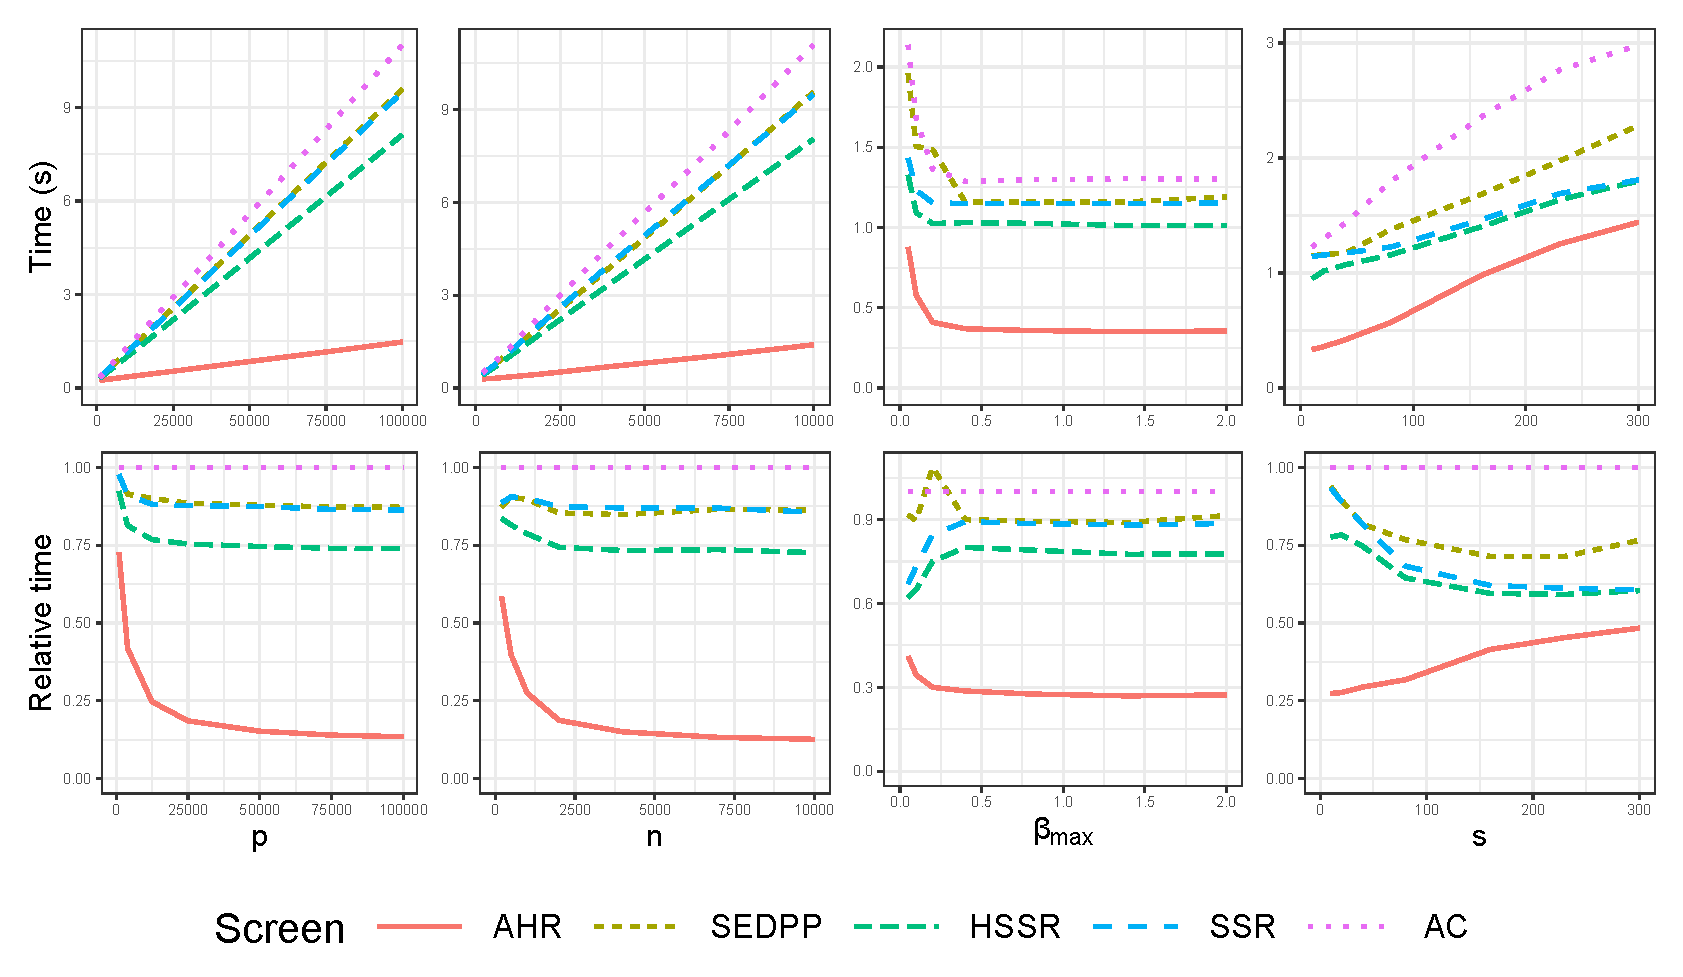
\includegraphics[width=\textwidth]{511.eps}    \caption{Comparing speed of screening methods for lasso model under different settings. Top row: computation time in second. Bottom row: relative computation time compared to AC. First column: varying number of features $p$. Second column: varying sample size $n$. Third column: varying signal strength $\beta_{\max}$. Fourth column: varying sparsity $s$.}
    \label{fig:5.1.1a}
\end{figure}

\begin{figure}[h]
    \centering
    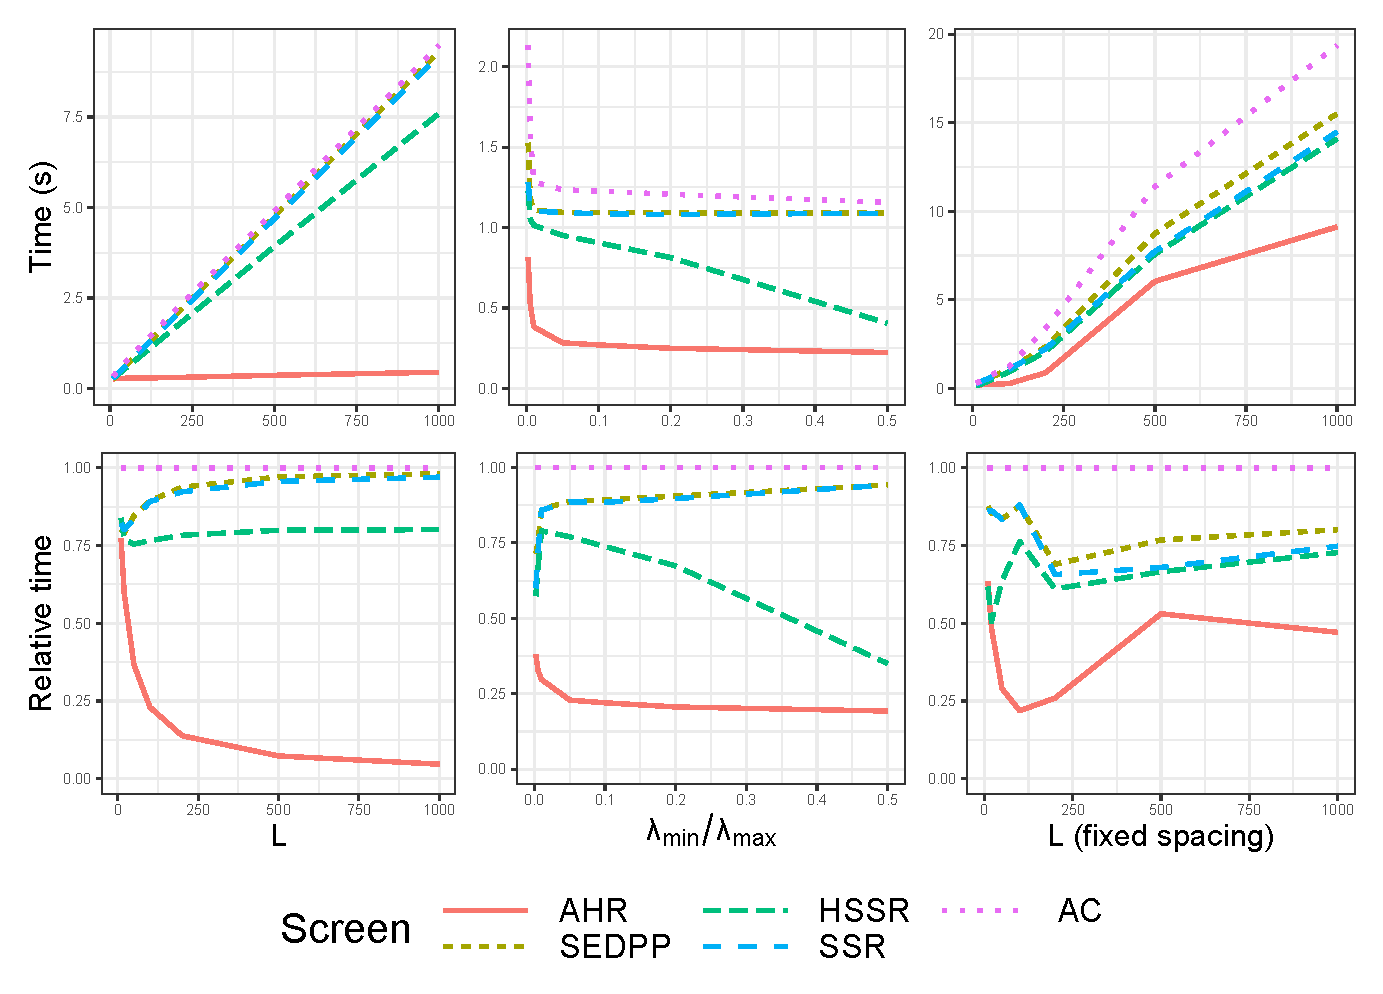
\includegraphics[width=0.82\textwidth]{511b.eps}    \caption{Comparing speed of screening methods for lasso model under different settings. Top row: computation time in second. Bottom row: relative computation time compared to AC. First column: Varying number of grid points $L$. Second column: Varying range of grid $\lambda_{\min}/\lambda_{\max}$. Third column: Varying number of grid points $L$ with fixed spacing.}
    \label{fig:5.1.1b}
\end{figure}

Figure~\ref{fig:5.1.1a} and~\ref{fig:5.1.1b} shows the computation time (top row) and relative computation time compared to AC (bottom row) of solving lasso problem with different screening methods. AHR is uniformly the fastest under all settings, typically 2-8 times faster than any other screening method. The difference is largest when the data set is large (large $n$ or large $p$), the active features are highly sparse (small $s$) or the grid of $\lambda$-value is fine (large $L$ or $\lambda_{\min}/\lambda_{\max}$). For example, when $L=1000$, AHR is 18 times faster than any other approach.

There are, however, cases when AHR's advantage over other methods is not as significant: (1) $p$ or $n$ is small. For small data sets, computation is less challenging and screening rules play a smaller role. (2) $\beta_{\max}$ is close to zero. When the nonzero coefficients are close to zero, they are hard to distinguish from each other. This tends to cause problems for any statistical learning method. (3) $s$ is large. In this case, the solution is \quotes{dense} and screening rules have less ability to leverage sparsity to computational advantage. (4) $L$ is small. In this case, only a coarse grid of $\lambda$-values are considered, providing less information for an adaptive approach to use. A practical downside to choosing a small $L$ is that the selected $\lam$ may be far from optimal.

We also tried varying other factors, for example: the correlation among features in $X$, sparsity with fixed signal strength, and the minimum value $\lambda_L$. The results of these experiments were very similar, with AHR continuing to show a uniform advantage over other methods.

\subsubsection{Sparse logistic Regression Model}

We now turn our attention to the sparse logistic regression model, comparing sequential strong rules (SSR), hybrid rules using Slores as the safe rule (HSlores), and adaptive screening using Slores as the safe rule (ASlores). SSR is implemented in all three methods and will be considered the baseline.

The data are simulated from the model: $y=\mathbf{1}\{X\beta+0.1\epsilon >0\}$. As before, $X$ and $\epsilon$ are sampled i.i.d from $N(0,1)$, while $\beta$ has $s$ randomly selected elements equally spaced between $[-\beta_{\max},\beta_{\max}]$. Each setting is replicated $10$ times to calculate the average time cost. We consider the same 7 cases as in the previous experiment.

\begin{figure}[h]
    \centering
    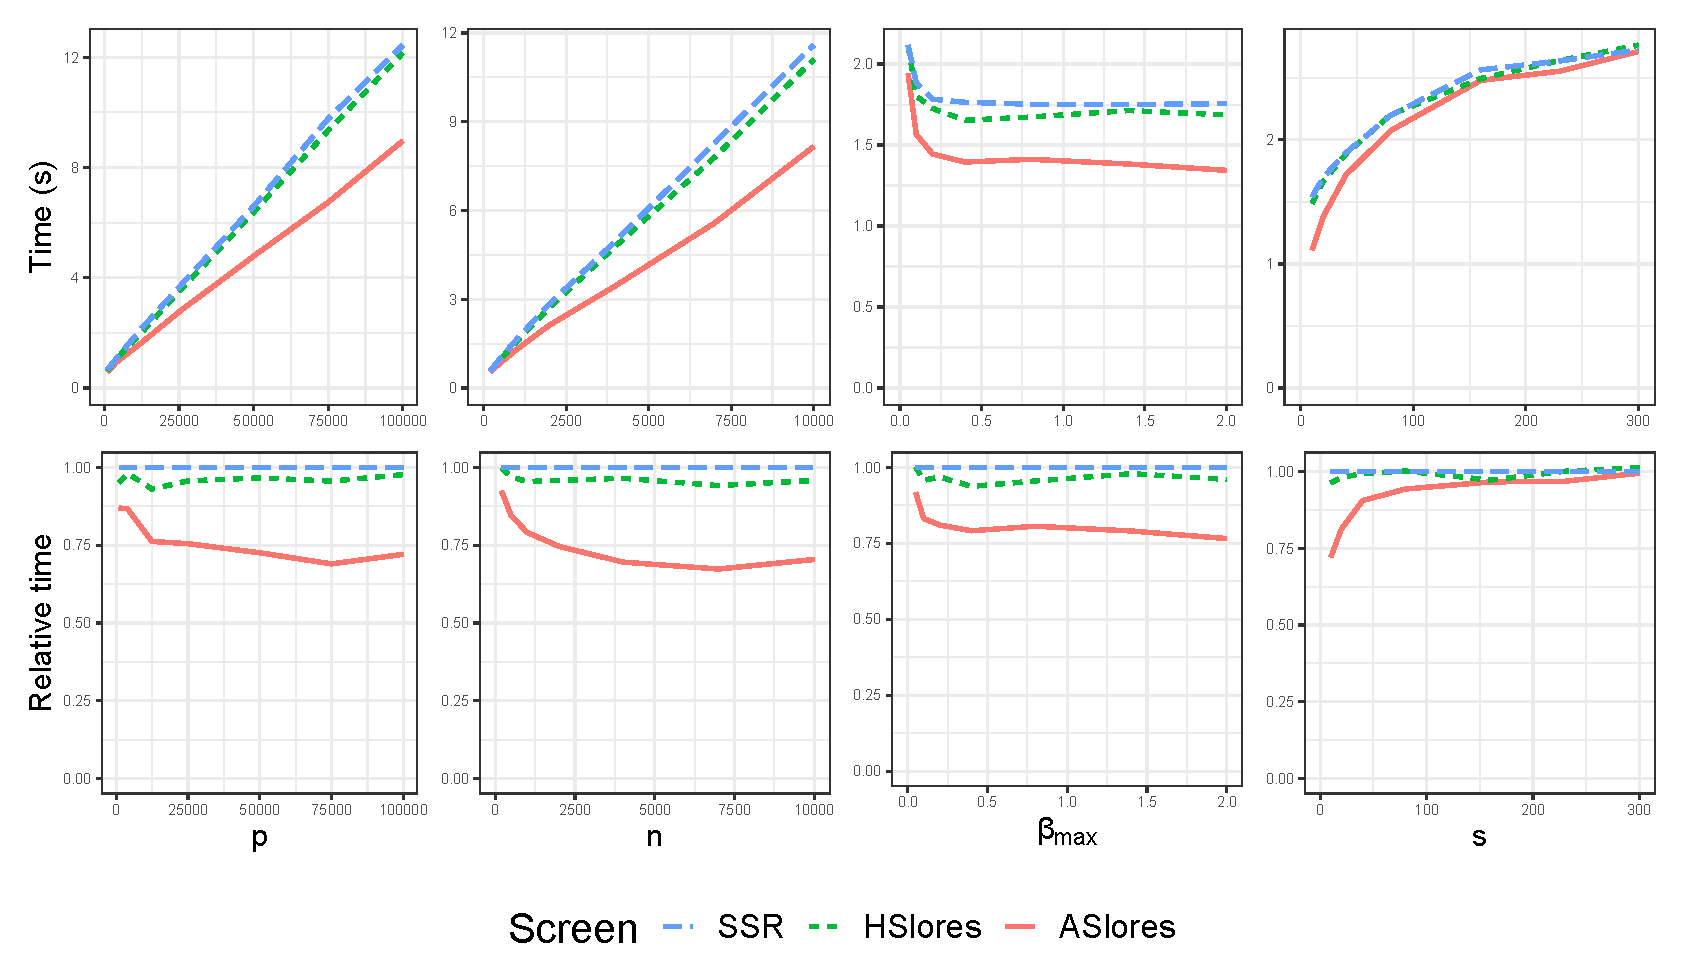
\includegraphics[width=\textwidth]{512.eps}    \caption{Comparing speed of screening methods for sparse logistic regression model under different settings. Top row: computation time in second. Bottom row: relative computation time compared to SSR. First column: varying number of features $p$. Second column: varying sample size $n$. Third column: varying signal strength $\beta_{\max}$. Fourth column: varying sparsity $s$.}
    \label{fig:5.1.2a}
\end{figure}

\begin{figure}[h]
    \centering
    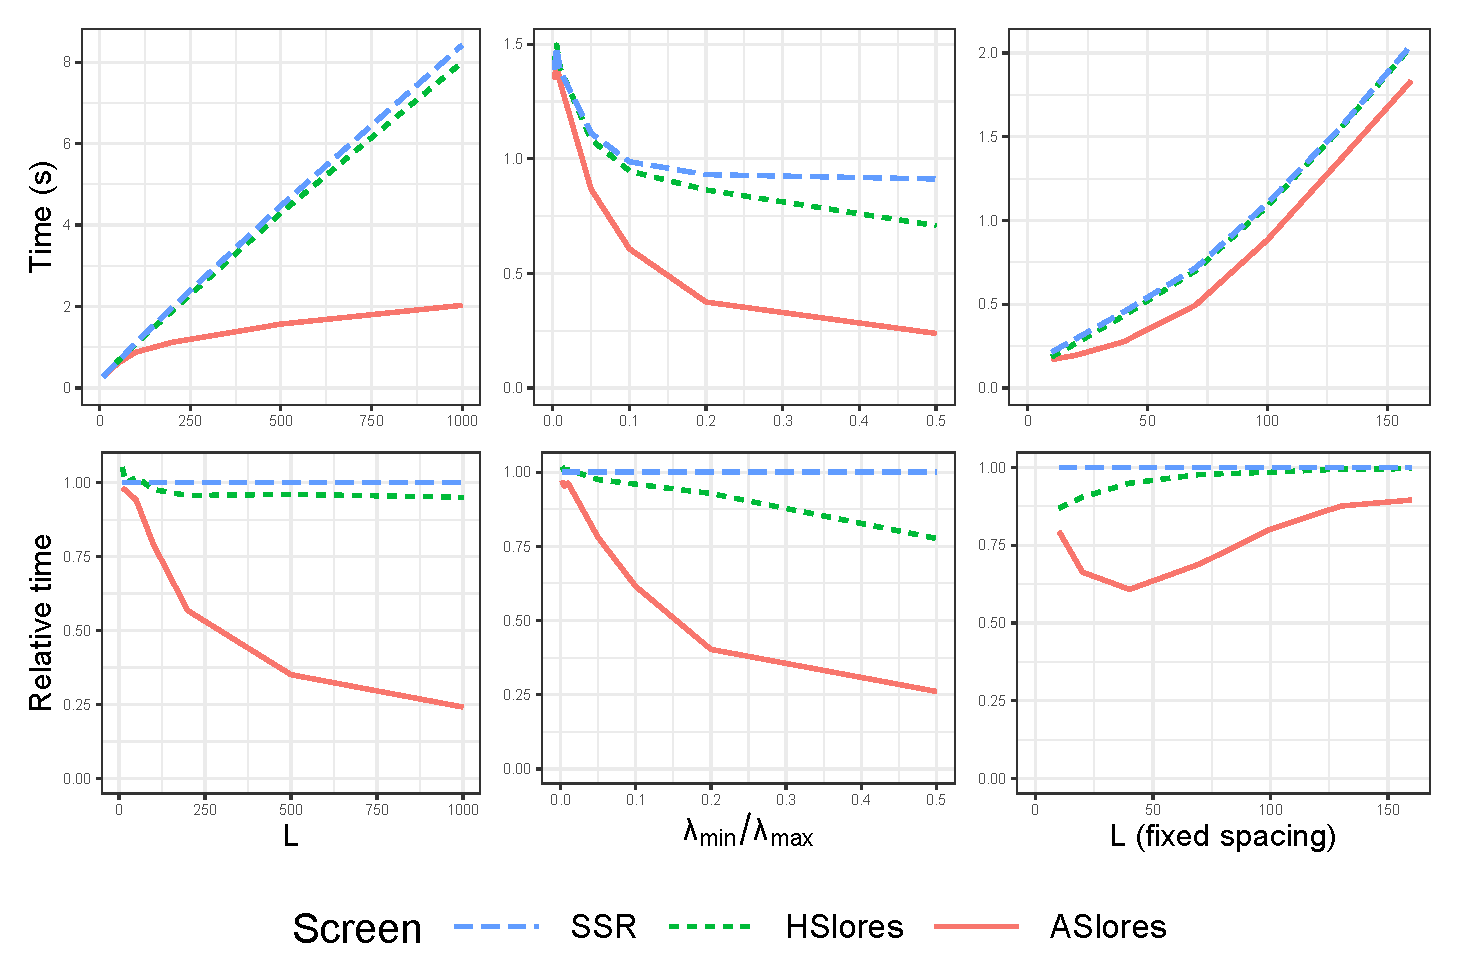
\includegraphics[width=0.82\textwidth]{512b.eps}    \caption{Comparing speed of screening methods for sparse logistic regression model under different settings. Top row: computation time in second. Bottom row: relative computation time compared to SSR. First column: Varying number of grid points $L$. Second column: Varying range of grid $\lambda_{\min}/\lambda_{\max}$. Third column: Varying number of grid points $L$ with fixed spacing.}
    \label{fig:5.1.2b}
\end{figure}

Figure~\ref{fig:5.1.2a} and~\ref{fig:5.1.2b} show the computation time (top row) and relative computation time compared to SSR (bottom row) of solving sparse logistic regression problem with different screening methods. The overall pattern is the same as for sparse linear regression, with adaptive screening uniformly faster than all other methods. The speedup is smaller in magnitude than for linear regression because the Slores rule is less powerful than EDPP. Nevertheless, the improvement in speed is still dramatic in many cases. For example, when $L=1,000$, AHR was 4 times faster than any other method.

\subsection{Real Data Analysis}
\label{sec:real-data}

The previous section compared screening methods under different scenarios using simulated data. Data generating mechanisms in the real world, however, are much more complex than those of a simulation. In this section, we compare screening methods for lasso models on a variety of real data sets to ensure the conclusions of the previous section are representative of real world data. Following the studies of \citep{wang2013lasso, xiang2016screening, Zeng2021}, we test the lasso screening methods on the following data sets:

\begin{enumerate}
    \item \textbf{Breast cancer gene expression data
(GENE, \url{https://myweb.uiowa.edu/pbreheny/data/bcTCGA.html}):} this data has expression measurements of $p=17,322$ genes from $n=536$ patients. The response is the expression measurement of the gene BRCA1, which has been identified to be related to risk of breast cancer.
    \item \textbf{MNIST handwritten image data
(MNIST, \url{http://yann.lecun.com/exdb/mnist}):} this data set has $60,000$ images in the training set and $10,000$ images in the testing set. Each image is a $28\times 28=784$ pixels image of handwritten digits. We use the training set to form a $n=784\times p=60,000$ feature matrix, treating pixels as samples and images as features. Then an image from the testing set is randomly selected as the response.
    \item \textbf{Cardiac fibrosis genome-wide association data
(GWAS, \url{https://arxiv.org/abs/1607.05636}):} this data set has $p=660,496$ single nucleotide
polymorphisms (SNPs) collected from $n=313$ human hearts. The response is the log of the ratio of cardiomyocytes to fibroblasts in the heart tissue, which is associated with heart failure.
    \item \textbf{Subset of New York Times bag-of-words data
(NYT, \url{https://archive.ics.uci.edu/ml/datasets/Bag+of+Words}):} the raw data set is a $300,000\times 102,660$ matrix, each row being a document and each column being number of occurrence of a specific word in those documents. We selected $n=5,500$ documents by removing documents with low word counts. Then $55,000$ words are selected as the features and a randomly selected word is the response.

\end{enumerate}


For GENE and GWAS, we replicate the experiment 10 times to take the average. For data sets MNIST and NYT, because the response is randomly selected, we replicate the experiment 50 times to get an accurate estimate. Table~\ref{Tab:real} compares the average computation time for different screening methods in these data sets.

\begin{table}[H]
\centering
\begin{tabular}{lllll}
\toprule
 & GENE & MNIST & GWAS & NYT \\
Screening method & n=536 & n=784 & n=313 & n=5,500 \\
       & p=17,322 & p=60,000 & p=660,496 & p=55,000 \\
\midrule
AC & 2.14 (0.03) & 6.82 (0.07) & 46.67 (0.13) & 59.20 (1.89) \\
SSR & 1.34 (0.01) & 5.20 (0.01) & 25.34 (0.08) & 35.40 (0.44) \\
SEDPP & 1.38 (0.01) & 8.40 (0.45) & 25.48 (0.05) & 53.69 (3.81) \\
HSSR & 1.21 (0.01) & 3.44 (0.07) & 23.85 (0.06) & 31.05 (0.80) \\
AHR & \textbf{0.71 (0.01)} & \textbf{1.15 (0.02)} & \textbf{8.80 (0.03)} & \textbf{12.71 (1.05)} \\
\bottomrule
\end{tabular}
\caption{Average computing time in second (standard error) for solving the lasso model}
\label{Tab:real}
\end{table}

AHR again outperforms other screening methods on all data sets, faster than other methods by factor ranging from 70\% to 630\%. Also note that the performance of SEDPP varies considerably for the MNIST and NYT data sets, where the response is randomly selected in each replication, indicating that the speed of SEDPP is sensitive to the data. AHR is built with SEDPP as the safe rule but does not share this issue of instability because it can adaptively adjust itself according the performance of the safe rule.

\subsection{Big Data Performance}

Ultra high dimensional big data that is too large to fit into memory represents the greatest challenge and the scenario where the help of a good screening method is needed most. To test the screening methods described in this paper, we used data from the Genetic Risk Assessment of Defibrillator Events study (GRADE, \url{https://www.clinicaltrials.gov/ct2/show/NCT02045043}). Genome-wide genetic data were collected for 1,080 subjects diagnosed with cardiomyopathy and who had undergone surgery to receive an implantable cardioverter defibrillator in the past 5 years. After imputation using the Haplotype Reference Consortium as a reference genome and filtering for quality control \citep{Das2016}, there were $p=11,830,470$ SNPs which used as features. The size of the file storing the feature matrix is 96G and we conduct the test on a machine with 32G RAM. We chose a relatively large $\lambda_{\min} =0.5\lambda_{\max}$ to avoid having more features selected than the number of observations, at which point the solution is no longer unique.

A variety of clinical data was collected on these individuals. To examine the performance of screening rules for linear regression, we focused on left ventricular ejection fraction (LVEF) as the response. LVEF measures the proportion of blood being pumped out of the left ventricle of the heart with each contraction. Lower values are associated with more severe heart disease. LVEF data was available for $n=973$ subjects and they will be considered as the sample for this analysis. The experiment is replicated 5 times, and results are shown in Table~\ref{Tab:lvef}.

\begin{table}[H]
\centering
\begin{tabular}{llllll}
\toprule
Screening method & AC\,\,\,\,\,\,\,\,\,    & SSR\,\,\,\,\,\,   & SEDPP & HSSR\,\,\,  & AHR\,\,\,\,\,\,  \\
\midrule
Time & 183.6 & 78.6 & 78.6 & 84.9 & 13.6 \\
Standard error & 0.43 & 0.65 & 0.20 & 0.48 & 0.15 \\
\bottomrule
\end{tabular}
\caption{Average computing time in minutes and standard error for the LVEF analysis (lasso-penalized linear regression).\label{Tab:lvef}}
\end{table}

For the sparse logistic model, we choose the New York Heart Association (NYHA) Functional Classification as the response, which classifies patients on the basis of limitations to their physical activity. The classes range from 1 to 4, which we dichotomize into patients with no or slight limitation of physical activity (classes 1 and 2) and patients with substantial limitations (classes 3 and 4). The NYHA classification was available for $n=1008$ subjects, who form the sample for the logistic regression analysis. The experiment is replicated 5 times to take the average and results are shown in Table~\ref{Tab:nyha}.

\begin{table}[H]
\centering
\begin{tabular}{llll}
\toprule
Screening method & SSR\,\,\,\,\,\,\,\,\,    & HSlores\,\,\,\,\,\,   & ASlores \\
\midrule
Time & 82.7 & 107.5 & 51.7 \\
Standard error & 0.10 & 0.67 & 0.17 \\
\bottomrule
\end{tabular}
\caption{Average computing time in minutes and standard error for the NYHA analysis (lasso-penalized logistic regression).\label{Tab:nyha}}
\end{table}

For both analyses, the proposed adaptive hybrid methods result in substantial reductions in computation time. In particular, for the lasso analysis of LVEF, the adaptive hybrid method reduces computation time from nearly an hour and a half to under 15 minutes, a 6-fold speedup.

\section{Conclusion}
\label{sec:6}

In this paper, we have proposed a novel adaptive hybrid screening framework for efficient lasso-type optimization over the solution path. The key idea is to judiciously reuse the reference for screening along the path until the point where updating to a new reference is beneficial.  We developed three instances of algorithms using this framework, for standard lasso-penalized linear regression, for sparse logistic regression, and for the group lasso. Extensive numeric experiments on both simulated and real data, including a very large data set that cannot fit into memory, demonstrate that our proposed algorithms outperform other state-of-the-art screening methods uniformly, in many cases several times faster that competing approaches.

The algorithms for lasso-penalized linear and logistic regression have been implemented in the publicly accessible R package \textbf{biglasso} \citep{zeng2017biglasso}, which was used to carry out the numeric experiments.

The proposed adaptive hybrid screening framework is flexible and can be extended in several ways. The framework is general and does not require a specific algorithm, strong rule, or safe rule. As faster algorithms to solve the lasso problem, better safe rules, or improved strong rules are developed, these can be directly plugged into the adaptive hybrid framework with a corresponding improvement in computational efficiency. Nevertheless, there are still several lasso type problems without sequential safe rules, such as sparse Cox regression, sparse Poisson regression, and sparse support vector machines. As safe rules for these problems are developed, they can be readily fit into our framework to produce efficient algorithms as well.

\renewcommand\bibname{References}
\bibliographystyle{tfnlm}
\begin{thebibliography}{10}
\providecommand{\url}[1]{\normalfont{#1}}
\providecommand{\urlprefix}{Available from: }

\bibitem{tibshirani1996regression}
Tibshirani~R. Regression shrinkage and selection via the lasso. Journal of the
  Royal Statistical Society: Series B (Methodological).
  1996;\hspace{0pt}58(1):267--288.

\bibitem{yuan2006model}
Yuan~M, Lin~Y. Model selection and estimation in regression with grouped
  variables. Journal of the Royal Statistical Society: Series B (Statistical
  Methodology). 2006;\hspace{0pt}68(1):49--67.

\bibitem{zou2005regularization}
Zou~H, Hastie~T. Regularization and variable selection via the elastic net.
  Journal of the Royal Statistical Society: Series B (Statistical Methodology).
  2005;\hspace{0pt}67(2):301--320.

\bibitem{friedman2007pathwise}
Friedman~J, Hastie~T, H{\"o}fling~H, et~al. Pathwise coordinate optimization.
  The Annals of Applied Statistics. 2007;\hspace{0pt}1(2):302--332.

\bibitem{Tibshirani2012}
Tibshirani~R, Bien~J, Friedman~J, et~al. Strong rules for discarding predictors
  in lasso-type problems. Journal of the Royal Statistical Society Series B.
  2012;\hspace{0pt}74(2):245--266.

\bibitem{qian2019fast}
Qian~J, Du~W, Tanigawa~Y, et~al. A fast and flexible algorithm for solving the
  lasso in large-scale and ultrahigh-dimensional problems. BioRxiv.
  2019;\hspace{0pt}:630079.

\bibitem{ghaoui2010safe}
Ghaoui~LE, Viallon~V, Rabbani~T. Safe feature elimination for the lasso and
  sparse supervised learning problems. arXiv:10094219. 2010;\hspace{0pt}.

\bibitem{wang2013lasso}
Wang~J, Zhou~J, Wonka~P, et~al. Lasso screening rules via dual polytope
  projection. In: Advances in Neural Information Processing Systems; 2013. p.
  1070--1078.

\bibitem{xiang2012fast}
Xiang~ZJ, Ramadge~PJ. Fast lasso screening tests based on correlations. In:
  International Conference on Acoustics, Speech and Signal Processing; IEEE;
  2012. p. 2137--2140.

\bibitem{xiang2011learning}
Xiang~ZJ, Xu~H, Ramadge~PJ. Learning sparse representations of high dimensional
  data on large scale dictionaries. In: Advances in Neural Information
  Processing Systems; 2011. p. 900--908.

\bibitem{Zeng2021}
Zeng~Y, Yang~T, Breheny~P. Hybrid safe–strong rules for efficient
  optimization in lasso-type problems. Computational Statistics \& Data
  Analysis. 2021;\hspace{0pt}153:107063.

\bibitem{zeng2017biglasso}
Zeng~Y, Breheny~P. The biglasso package: a memory-and computation-efficient
  solver for lasso model fitting with big data in {R}. arXiv:170105936.
  2017;\hspace{0pt}.

\bibitem{lee2007efficient}
Lee~H, Battle~A, Raina~R, et~al. Efficient sparse coding algorithms. In:
  Advances in neural information processing systems; 2007. p. 801--808.

\bibitem{Fan2008}
Fan~J, Lv~J. Sure independence screening for ultrahigh dimensional feature
  space. Journal of the Royal Statistical Society Series B.
  2008;\hspace{0pt}70(5):849--911.

\bibitem{wang2014safe}
Wang~J, Zhou~J, Liu~J, et~al. A safe screening rule for sparse logistic
  regression. In: Advances in Neural Information Processing Systems; 2014. p.
  1053--1061.

\bibitem{breheny2015group}
Breheny~P, Huang~J. Group descent algorithms for nonconvex penalized linear and
  logistic regression models with grouped predictors. Statistics and Computing.
  2015;\hspace{0pt}25(2):173--187.

\bibitem{xiang2016screening}
Xiang~ZJ, Wang~Y, Ramadge~PJ. Screening tests for lasso problems. IEEE
  Transactions on Pattern Analysis and Machine Intelligence.
  2016;\hspace{0pt}39(5):1008--1027.

\bibitem{Das2016}
Das~S, Forer~L, Sch{\"o}nherr~S, et~al. Next-generation genotype imputation
  service and methods. Nature Genetics. 2016 Oct;\hspace{0pt}48(10):1284--1287.

\end{thebibliography}

\end{document}
